\documentclass[tikz,border=10pt]{standalone}
\usetikzlibrary{intersections, calc}

\begin{document}
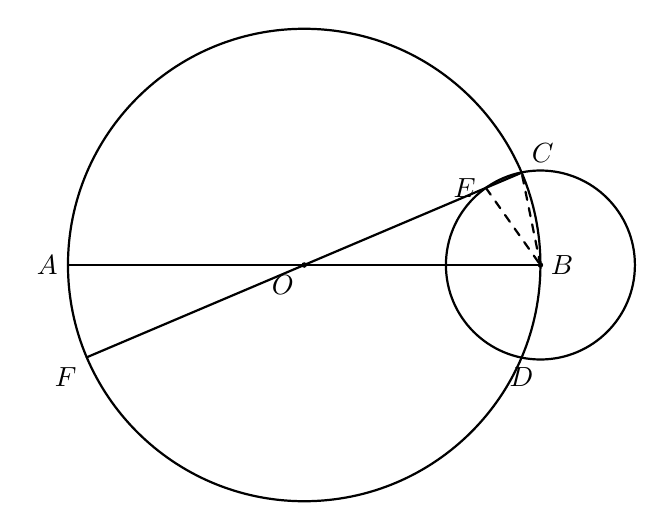
\begin{tikzpicture}[line cap=round, line join=round, >=stealth, thick]

    % --- 参数定义 ---
    \def\R{3}    % 大圆半径
    \def\r{1.2}  % 小圆半径
    
    % --- 坐标定义 ---
    \coordinate (O) at (0,0);           % 大圆圆心
    \coordinate (B) at (\R,0);          % 小圆圆心，位于大圆右边缘
    \coordinate (A) at (-\R,0);         % 大圆左边缘点
    
    % --- 绘制圆 ---
    % 绘制大圆 (Circle O)
    \draw[name path=circleO] (O) circle (\R);
    % 绘制小圆 (Circle B)
    \draw[name path=circleB] (B) circle (\r);
    
    % --- 计算交点 ---
    % 计算两圆交点 C 和 D
    \fill [name intersections={of=circleO and circleB, by={C,D}}];
    
    % 定义经过 O 的斜线 (根据原图角度，设定约为 30 度)
    \def\angleF{203} % F点在大圆上的极角
    \coordinate (F) at (\angleF:\R);
    \coordinate (E_tmp) at (\angleF+180:\R); % 对角线方向点
    
    % 绘制直线 F-O 向右上方延伸
    \draw[name path=lineFE] (F) -- ($(O)!1!(E_tmp)$);
    
    % 计算直线与小圆的交点 E 和 C' (图中 E 点在小圆靠近圆心方向)
    \fill [name intersections={of=lineFE and circleB, by={E,C_prime}}];

    % --- 绘制直线 ---
    \draw (A) -- (B); % 水平直径线
    \draw[dashed] (E) -- (B);
     \draw[dashed] (B) -- (C);
    
    % --- 标注点 ---
    \fill (O) circle (1pt) node[below left] {$O$};
    \fill (B) circle (1pt) node[right] {$B$};
    
    % 文本标签标注 (根据原图视觉位置微调)
    \node[left] at (A) {$A$};
    \node[below left] at (F) {$F$};
    \node[left] at (E) {$E$};
    \node[above right] at (C) {$C$};
    \node[below] at (D) {$D$};

\end{tikzpicture}
\end{document}